% =====================================================================
%  ARTIGO -- Projeto do Capítulo 3: a vizinhança solar com o Gaia
%  Astronomia (AST0001) -- Curso de Física -- UDESC Joinville
%
%  Esqueleto do artigo do projeto do Gaia, no modelo de artigo da
%  disciplina. Diferente dos laboratórios dos outros capítulos, aqui as
%  figuras e as tabelas são SUAS: você as produz no Excel ou no Python a
%  partir do arquivo 01_gaia_estrelas_25pc.csv. Os lugares já estão
%  marcados e referenciados no texto.
%
%  COMO USAR
%   1. Preencha os campos marcados "PREENCHA AQUI".
%   2. Escreva nas seções indicadas, apagando as instruções.
%   3. Compile com pdfLaTeX DUAS vezes (a segunda resolve as referências).
% =====================================================================

\documentclass[10pt,a4paper,twocolumn]{article}

\usepackage[utf8]{inputenc}
\usepackage[T1]{fontenc}
\usepackage[brazil]{babel}
\usepackage{amsmath,amssymb}
\let\Bbbk\relax
\usepackage{newtxtext,newtxmath}
\usepackage{microtype}
\usepackage[a4paper,top=2.4cm,bottom=2.2cm,left=1.9cm,right=1.9cm,
            columnsep=0.7cm]{geometry}
\usepackage{graphicx}
\usepackage{booktabs}
\usepackage{siunitx}
\usepackage{caption}
\usepackage{titlesec}
\usepackage{fancyhdr}
\usepackage{xcolor}
\usepackage[colorlinks=true,linkcolor=udescverde,citecolor=udescverde,
            urlcolor=udescverde]{hyperref}

\definecolor{udescverde}{HTML}{1B6B3A}
\definecolor{cinza}{HTML}{5A5A5A}

\sisetup{output-decimal-marker={,}, per-mode=symbol}

\captionsetup{font=small,labelfont={bf,color=udescverde},labelsep=period}
\titleformat{\section}{\normalfont\bfseries\color{udescverde}}
            {\thesection.}{0.5em}{\MakeUppercase}
\titleformat{\subsection}{\normalfont\bfseries\itshape}{\thesubsection.}{0.5em}{}
\titlespacing*{\section}{0pt}{1.6ex}{0.8ex}
\setlength{\parindent}{1.2em}

% usado pelas tabelas que o laboratório gerou
\newcommand{\compacttables}{\footnotesize\setlength{\tabcolsep}{3pt}}

% ---------------------------------------------------- PREENCHA AQUI
\newcommand{\titulo}{A densidade estelar da vizinhança solar medida com o Gaia}
\newcommand{\autores}{PREENCHA: Nome Um, Nome Dois, Nome Três}
% um endereço por autor, na mesma ordem dos nomes
\newcommand{\emails}{aluno1@edu.udesc.br, aluno2@edu.udesc.br, aluno3@edu.udesc.br}
% aparece no cabeçalho das páginas; troquem se preferirem outra forma
\newcommand{\autoresCurto}{PREENCHA: Sobrenome et al.}
\newcommand{\tituloCurto}{Densidade da vizinhança solar}
\newcommand{\semestre}{2026/2}
% -------------------------------------------------------------------

\pagestyle{fancy}
\fancyhf{}
\fancyhead[L]{\footnotesize\textcolor{cinza}{\autoresCurto}}
\fancyhead[R]{\footnotesize\textcolor{cinza}{\tituloCurto}}
\fancyfoot[C]{\footnotesize\textcolor{cinza}{\thepage}}
\renewcommand{\headrulewidth}{0.3pt}
\fancypagestyle{primeira}{%
  \fancyhf{}\renewcommand{\headrulewidth}{0pt}
  \fancyfoot[C]{\footnotesize\textcolor{cinza}{\thepage}}}

\begin{document}

\twocolumn[
\begin{@twocolumnfalse}

\noindent
\begin{minipage}{0.78\textwidth}
  {\footnotesize\textcolor{udescverde}{\textbf{ASTRONOMIA (AST0001)}}\\[2pt]
   \textcolor{cinza}{Universidade do Estado de Santa Catarina\, $\cdot$\,
   Centro de Ciências Tecnológicas\, $\cdot$\, Curso de Física}\\[2pt]
   \textcolor{cinza}{Joinville, \semestre}}
\end{minipage}
\hfill
\begin{minipage}{0.20\textwidth}
  \raggedleft{
\includegraphics[height=1.5cm]{udesc.png}}
\end{minipage}

\vspace{2pt}
{\color{udescverde}\rule{\textwidth}{1pt}}

\vspace{1.1em}
\begin{center}
  {\LARGE\bfseries \titulo\par}
  \vspace{0.9em}
  {\large \autores\par}
  \vspace{0.3em}
  {\footnotesize\itshape\textcolor{cinza}{\emails}\par}
  \vspace{0.3em}
  {\footnotesize\textcolor{cinza}{Recebido em \today}\par}
\end{center}

\vspace{0.9em}

% ------------------------------------------------------------ RESUMO
% Um parágrafo, de 120 a 200 palavras: contexto em uma frase, o que foi
% feito, que dados, o RESULTADO NUMÉRICO com incerteza, e a conclusão em
% uma frase. Escrito por último, lido primeiro. Sem citar figuras.
\noindent\rule{\textwidth}{0.3pt}
\vspace{0.5em}

{\small
\noindent\textbf{Resumo.}
Escreva aqui, por último. Diga que usou um catálogo do Gaia com as 2000
estrelas mais próximas do Sol, que validou até que raio a amostra é completa,
e que dentro desse raio contou objetos para obter a densidade estelar local.
Apresente o resultado principal em números, com incerteza:
$n = \underline{\hspace{2.2em}} \pm \underline{\hspace{1.6em}}\ \mathrm{pc^{-3}}$,
contra cerca de $0{,}10\,\mathrm{pc^{-3}}$ do censo de referência. Diga em uma
frase o que explica a diferença --- ela não é erro de medida.

\vspace{0.6em}
\noindent\textbf{Palavras-chave:} astronomia estelar --- paralaxe ---
amostra limitada por volume --- densidade estelar
}

\vspace{0.5em}
\noindent\rule{\textwidth}{0.3pt}
\vspace{1.4em}

\end{@twocolumnfalse}
]
\thispagestyle{primeira}

% =====================================================================
\section{Introdução}
% =====================================================================
% O que e uma amostra limitada por VOLUME, e por que ela e rara.
% A maior parte dos catalogos e limitada por MAGNITUDE: enxerga longe as
% estrelas brilhantes e perto as fracas, e por isso nao serve para contar.
% A vizinhanca solar e o unico lugar onde se consegue algo proximo de um
% censo completo -- e mesmo ali, com as falhas que a Secao 4 discute.

Escreva aqui.

% =====================================================================
\section{Revisão Teórica}
% =====================================================================
% So o que voce usou, com as hipoteses ditas em voz alta.

A paralaxe dá a distância por geometria pura,
\begin{equation}
d\,[\mathrm{pc}] = \frac{1000}{p\,[\mathrm{mas}]} ,
\label{eq:dist}
\end{equation}
e a distância converte brilho aparente em brilho intrínseco pelo módulo de
distância,
\begin{equation}
M = m - 5\log_{10} d + 5 .
\label{eq:modulo}
\end{equation}
Uma contagem dentro de um volume dá a densidade, e a incerteza de uma contagem
de eventos independentes é de Poisson:
\begin{equation}
n = \frac{N}{\tfrac{4}{3}\pi R^{3}} ,
\qquad
\frac{\sigma_n}{n} = \frac{1}{\sqrt{N}} .
\label{eq:dens}
\end{equation}
% ATENCAO: a Eq. (1) e exata para os valores VERDADEIROS. Para valores
% medidos ela e enviesada -- veja a secao "O vies de inverter a paralaxe",
% no Capitulo 3. Diga aqui por que, NESTA amostra, inverter e legitimo.

% =====================================================================
\section{Dados}
% =====================================================================
% Origem, colunas usadas, e -- obrigatorio -- os limites da amostra.

Escreva aqui: qual arquivo, quantas estrelas, quais colunas foram usadas.

\textbf{Limites da amostra.} Três características precisam entrar em qualquer
resultado tirado daqui, e a Seção~\ref{sec:disc} volta a elas:
\begin{enumerate}\itemsep2pt
\item o raio real da amostra não é o do nome do arquivo --- determine-o pela
      menor paralaxe e diga qual é;
\item faltam as estrelas mais brilhantes, porque o Gaia satura;
\item uma fração das estrelas não tem velocidade radial medida, e planilha
      trata célula vazia como zero.
\end{enumerate}

% =====================================================================
\section{Resultados}
% =====================================================================
% Numeros e graficos. Interpretacao fica na Discussao.

\begin{figure}[t]
\centering
% troque pelo SEU diagrama, exportado do Excel ou do matplotlib
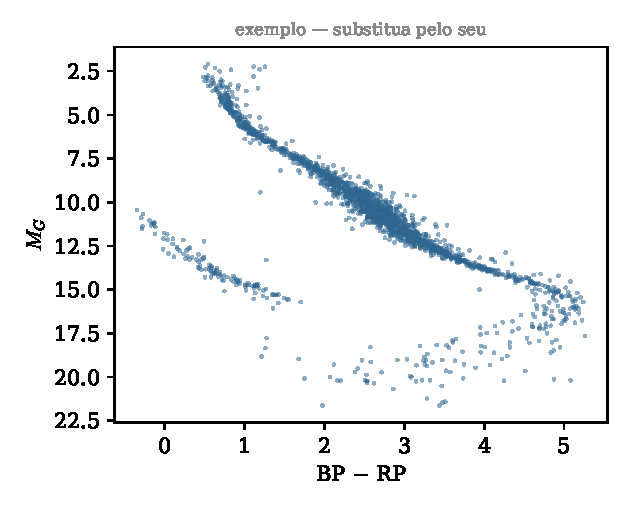
\includegraphics[width=\columnwidth]{figuras/diagrama_hr.pdf}
\caption{Diagrama cor--magnitude das estrelas da amostra: $M_G$ contra
$\mathrm{BP}-\mathrm{RP}$, com o eixo vertical invertido. Indique na legenda
os dois grupos e \textbf{declare o critério} que separou um do outro.}
\label{fig:hr}
\end{figure}

\begin{figure}[t]
\centering
% troque pelo SEU grafico de completeza
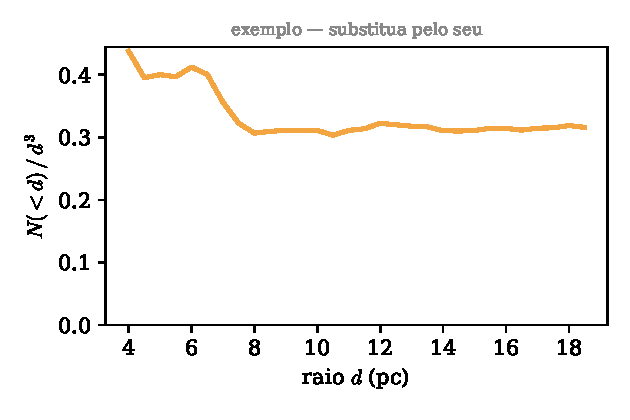
\includegraphics[width=\columnwidth]{figuras/completeza.pdf}
\caption{Teste de completeza: $N(<d)/d^{3}$ contra $d$. Enquanto a curva está
plana, a amostra contém tudo o que existe até ali. Marque o raio em que ela
deixa de ser plana --- é o maior raio que se pode usar na Eq.~\eqref{eq:dens}.}
\label{fig:completeza}
\end{figure}

Escreva aqui, apoiando-se na Tabela~\ref{tab:resultados}.

\begin{table}[t]
\centering\footnotesize
\caption{Resultados. Preencha com os seus números; a última coluna é a
referência da literatura, quando existir.}
\label{tab:resultados}
\begin{tabular}{lrr}
\toprule
grandeza & medido & referência \\
\midrule
raio de completeza $R$ (pc)            &  & --- \\
estrelas dentro de $R$                 &  & --- \\
densidade $n$ (pc$^{-3}$) &  & $\sim0{,}10$ \\
anãs brancas (\%)                      &  & --- \\
maior movimento próprio ($^{\prime\prime}$/ano) &  & --- \\
\bottomrule
\end{tabular}
\end{table}

% =====================================================================
\section{Discussão}
\label{sec:disc}
% =====================================================================
% Aqui esta a nota. Tres coisas que este projeto cobra:
%
%  (a) A diferenca entre o seu n e o valor de referencia NAO e erro: e
%      deficit de deteccao. Nomeie cada efeito -- anas marrons ausentes,
%      companheiras nao resolvidas, corte de brilho -- e, quando possivel,
%      estime o tamanho de cada um.
%
%  (b) O criterio que voce usou para separar as anas brancas muda a
%      contagem. Diga qual foi, e o que mudaria com outro.
%
%  (c) Ordene por velocidade espacial e olhe as maiores ANTES de usa-las.
%      Algumas sao fisicamente implausiveis. Diga o que fez com elas e por
%      que -- descartar sem dizer nao vale, e manter sem comentar, menos
%      ainda.

Escreva aqui.

% =====================================================================
\section{Conclusão}
% =====================================================================
% Tres a cinco frases: o que foi medido, com que numero e que incerteza, e
% o que dominaria uma medida melhor.

Escreva aqui.

% =====================================================================
\section*{Referências}
% =====================================================================

\begin{thebibliography}{9}\footnotesize
\bibitem{gaia} GAIA COLLABORATION. \emph{Gaia Data Release 3}. Astronomy \&
Astrophysics, 2023.
\bibitem{apostila} LIMA, R. C. R. \emph{Astrofísica Moderna: apostila de
capítulos de estudo}. UDESC Joinville, 2026. Capítulo 3.
\bibitem{censo} PREENCHA: a fonte do valor de referência da densidade local.
\end{thebibliography}

\end{document}
